% ---------------------------------------------------------------------------- %

\section{Funcionalidades}
\label{sec:func}

Nesta secção enumeram-se as funcionalidades disponibilizadas pelo sistema \SYS, detalhando-se depois o modo de utilização da interface de linha de comandos do mesmo.

% ---------------------------------------------------------------------------- %

\subsection{Funcionalidades disponibilizadas}

O sistema \SYS permite realizar transferências de ficheiros entre \nonpt{peers}, cada um exportando uma sub-árvore de um sistema de ficheiros local através de um \nonpt{socket} UDP (cf. Figura~\ref{fig:func:arch}). As transferências de ficheiros são depois realizadas entre as várias sub-árvores exportadas pelos \nonpt{peers} envolvidos. Transferências em ambos os sentidos (\emph{i.e.}, \nonpt{download} e \nonpt{upload}) podem ser iniciadas por qualquer \nonpt{peer}. O sistema disponibiliza todas as funcionalidades exigidas pelo enunciado do trabalho, expondo ainda várias funcionalidades adicionais.

\begin{figure}[ht]
  \centering
  \vspace*{.1\baselineskip}
  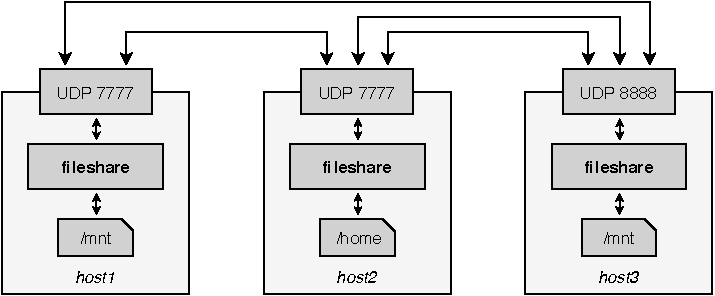
\includegraphics{figures/arch.pdf}
  \caption{Arquitetura \nonpt{peer-to-peer} do sistema \SYS.}
  \label{fig:func:arch}
  \vspace*{-.7\baselineskip}
\end{figure}

\itemizedpar{Aceitação de pedidos de transferência.}

Cada \nonpt{peer} define, com recurso a uma \nonpt{whitelist}, quais os \nonpt{peers} que podem ter acesso à sub-árvore local exportada, tanto para transferências de \nonpt{download} como de \nonpt{upload}. Esta \nonpt{whitelist} consiste num conjunto de intervalos de endereços IPv4 e IPv6 em notação CIDR. Ao se receber um pedido de transferência, este apenas é aceite se o endereço do \nonpt{peer} que realizou o pedido pertencer a algum dos intervalos de endereços na \nonpt{whitelist}.

\itemizedpar{Transferências de \nonpt{download}.}

Um \nonpt{peer} pode obter um ficheiro a partir de um ou mais outros \nonpt{peers} realizando uma transferência de \nonpt{download}. O utilizador deve especificar o caminho para o ficheiro a ser obtido (relativo às raizes das sub-árvores exportadas pelos \nonpt{peers} remotos) e os endereços dos \nonpt{peers} a partir dos quais o ficheiro deve ser transferido. Pode-se ainda especificar o caminho do ficheiro local resultante da transferência, caso não se deseje utilizar o mesmo caminho que o do ficheiro remoto.

Caso o utilizador indique que deve ser utilizado mais de um \nonpt{peer} remoto para se realizar a transferência, o ficheiro é dividido em segmentos de tamanho igual e cada segmento é obtido de um \nonpt{peer} distinto, em paralelo. Neste caso é também verificado que todos os \nonpt{peers} reportam o mesmo tamanho de ficheiro.

\itemizedpar{Transferências de \nonpt{upload}.}

Cada \nonpt{peer} pode também enviar um ficheiro para um ou mais outros \nonpt{peers} iniciando uma transferência de \nonpt{upload}. O utilizador especifica o caminho para o ficheiro a ser enviado (relativo à raiz da sub-árvore exportada pelo \nonpt{peer} local) e os endereços dos \nonpt{peers} para os quais o ficheiro deve ser transferido. É ainda possível indicar o caminho do ficheiro remoto resultante da transferência, ao invés de se utilizar o mesmo caminho que o do ficheiro local.

Caso o utilizador indique mais de um \nonpt{peer} remoto, o ficheiro é transmitido em paralelo e na sua totalidade para cada um dos \nonpt{peers}.

\itemizedpar{Transferências concorrentes.}

O sistema permite realizar qualquer número transferências em simultâneo entre qualquer par de \nonpt{peers}, incluindo combinações de transferências de \nonpt{download} e \nonpt{upload}. Cada \nonpt{peer} garante que o mesmo ficheiro não é modificado concorrentemente por mais de uma transferência, permitindo no entanto acessos de leitura simultâneos.

Nota-se também que, ao se receber um ficheiro (seja por se ter requerido uma transferência de \nonpt{download} ou por se servir um pedido de transferência de \nonpt{upload}), as alterações a esse ficheiro apenas são tornadas visíveis se a transferência for realizada com sucesso na sua totalidade. Em particular, se um ficheiro com o mesmo caminho já existir, este não é alterado caso a transferência falhe ou não termine com sucesso.

% ---------------------------------------------------------------------------- %

\subsection{Interface de linha de comandos}

O sistema \SYS é constituído por um único programa (ficheiro \path{fileshare.jar} no arquivo \ARQUIVO disponibilizado juntamente com este relatório), o qual permite iniciar um \nonpt{peer} local e executar transferências utilizando outros \nonpt{peers}. O programa disponibiliza uma interface de linha de comandos e tem a seguinte forma de invocação:

\begin{minted}{bash}
    fileshare [-a|--allow-all] [-p|--port <n>] <export_dir>
\end{minted}

O argumento \verb|<export_dir>| especifica a raiz da sub-árvore de sistema de ficheiros local a ser exportada pelo \nonpt{peer}, devendo ser um caminho para uma diretoria. As opções têm os seguintes significados:

\begin{itemize}

    \item \verb|-a| ou \verb|--allow-all| --- especifica que qualquer outro \nonpt{peer} pode realizar transferências utilizando o \nonpt{peer} local;
    
    \item \verb|-p <n>| ou \verb|--port <n>| --- especifica a porta UDP local que o \nonpt{peer} deve utilizar (se esta opção não for dada, a porta 7777 é selecionada).

\end{itemize}

O programa disponibiliza um \nonpt{prompt} interativo onde o utilizador pode introduzir comandos com o objetivo de realizar transferências de ficheiros entre \nonpt{peers}. Para executar o programa, recomenda-se a utilização do \nonpt{script} \path{fileshare.sh} (incluído também no arquivo \ARQUIVO), o qual expõe o mesmo modo de utilização mas adiciona funcionalidades de histórico de comandos ao \nonpt{prompt} interativo.

O \nonpt{prompt} interativo disponibiliza os seguintes comandos:

\newcommand{\comando}[1]{\textbf{\texttt{#1}}}

\newcommand{\comandodesc}[3]{%
  \begin{description}[style=nextline]%
  \item[\textbf{\texttt{#1 }\mintinline{bash}{#2}}]%
  #3%
  \end{description}%
  }

\comandodesc{exit}{}{Termina o \nonpt{peer} local e sai do \nonpt{prompt} interativo. Equivalente a fechar a \nonpt{stream} de \nonpt{standard input} através da combinação de teclas Ctrl+D.}

\comandodesc{whitelist-add}{<cidr_peers...>}{Adiciona os padrões de endereços em notação CIDR especificados (separados por espaços) à \nonpt{whitelist} de endereços de \nonpt{peers}.}

\comandodesc{whitelist-remove}{<cidr_peers...>}{Remove os padrões de endereços em notação CIDR especificados (separados por espaços) da \nonpt{whitelist} de endereços de \nonpt{peers}.}

\comandodesc{whitelist-all}{}{Adiciona os padrões \path{0.0.0.0/0} e \path{::/0} à \nonpt{whitelist} de endereços de \nonpt{peers}, permitindo que qualquer outro \nonpt{peer} realize transferências utilizando o \nonpt{peer} local. Equivalente a se especificar a opção \texttt{-a} ou \texttt{--allow-all} ao se invocar o programa.}

\comandodesc{whitelist-clear}{}{Remove todos os padrões de endereços da \nonpt{whitelist} de endereços de \nonpt{peers}.}

\comandodesc{get}{<remote_file> [as <local_file>] from <peers...>}{Realiza o \nonpt{download} do ficheiro com o caminho \texttt{<remote\_file>} a partir dos \nonpt{peers} com endereços \texttt{<peers...>} (separados por espaços), armazenando-o com o caminho \texttt{<local\_file>} (ou, se não especificado, com o caminho \texttt{<remote\_file>}). Se for dado mais de um \nonpt{peer}, a transferência é particionada e realizada em simultâneo a partir deles.}

\comandodesc{put}{<local_file> [as <remote_file>] to <peers...>}{Realiza o \nonpt{upload} do ficheiro com o caminho \texttt{<local\_file>} para os \nonpt{peers} com endereços \texttt{<peers...>} (separados por espaços), armazenando-o com o caminho \texttt{<remote\_file>} (ou, se não especificado, com o caminho \texttt{<local\_file>}). Se for dado mais de um \nonpt{peer}, a transferência é realizada em simultâneo para todos eles.}

\comandodesc{concurrent}{}{Permite realizar qualquer número e tipo de transferências em simultâneo. Execuções de \comando{get} e \comando{put} após a utilização deste comando apenas são realizadas ao se introduzir o comando \comando{run}, após o qual se regressa ao modo de execução imediata de transferências. O comando \comando{cancel} pode ser utlizado para se cancelar a realização de transferências já introduzidas e se voltar ao modo de execução imediata.}

% ---------------------------------------------------------------------------- %

\subsection{Exemplos de utilização}

Apresentam-se de seguida exemplos de utilização do programa \path{fileshare} e dos comandos do \nonpt{prompt} interativo disponibilizado pelo mesmo.

\begin{itemize}[noitemsep]

    \item Inicia um \emph{peer} na porta 8888, exportando a diretoria \path{/mnt}, e adiciona os intervalos de endereços \path{192.168.1.0/24} e \path{193.137.0.0/16} à \nonpt{whitelist}, ficando apto para servir transferências de ficheiros requeridas por \emph{peers} cujos endereços estejam contidos em algum de ambos esses intervalos.

    \vspace*{.9\baselineskip}
    \begin{Verbatim}[breaklines,gobble=8,frame=leftline,framesep=8pt,xleftmargin=11pt,commandchars=\\\{\}]
        \textcolor{Blue}{$} fileshare -p 8888 /mnt
        Exporting directory "/mnt" through UDP port 8888.
        \textcolor{RoyalBlue}{>} whitelist-add 192.168.1.0/24 193.137.0.0/16
        \textcolor{RoyalBlue}{>}
    \end{Verbatim}
    \vspace*{.9\baselineskip}

    \item Inicia um \nonpt{peer} na porta 7777, exportando a diretoria \path{/mnt}, e realiza o \nonpt{download} do ficheiro \path{file-1} a partir dos \nonpt{peers} com endereços \path{192.168.1.123}, \path{192.168.1.234} e \path{172.157.2.167}, e portas 7777, 12345 e 7777, respetivamente. No exemplo, a transferência está em progresso, tendo-se já recebido 63\% do ficheiro.

    \vspace*{.9\baselineskip}
    \begin{Verbatim}[breaklines,gobble=8,frame=leftline,framesep=8pt,xleftmargin=11pt,commandchars=\\\{\}]
        \textcolor{Blue}{$} fileshare /mnt
        Exporting directory "/mnt" through UDP port 7777.
        \textcolor{RoyalBlue}{>} get file-1 from 192.168.1.123 192.168.1.234:12345 172.157.2.167
        \textcolor{YellowOrange}{[ 63\%]} Getting file-1 from 3 peers... (9673.28 KiB/s)
    \end{Verbatim}
    \vspace*{.9\baselineskip}

    \item Inicia um \nonpt{peer} na porta 7777, exportando a diretoria \path{/mnt}, e realiza, concorrentemente, \inlineenum{1} o \nonpt{download} do ficheiro \path{file-2} a partir do \nonpt{peer} com \nonpt{hostname} \path{host123} e porta 8888, e \inlineenum{2} o \nonpt{upload} do ficheiro \path{my-things/file-3} para o \nonpt{peer} com \nonpt{hostname} \path{host123} e para o \nonpt{peer} com endereço \path{172.157.2.167}, ambos na porta 7777, e com o nome \path{another-name} nos \nonpt{peers} de destino. A primeira transferência falhou devido ao \nonpt{peer} remoto rejeitar a conecção (o endereço local não pertence à \nonpt{whitelist} desse \nonpt{peer}). A segunda transferência terminou com sucesso.

    \vspace*{.9\baselineskip}
    \begin{Verbatim}[breaklines,gobble=8,frame=leftline,framesep=8pt,xleftmargin=11pt,commandchars=\\\{\}]
        \textcolor{Blue}{$} fileshare /mnt
        Exporting directory "/mnt" through UDP port 7777.
        \textcolor{RoyalBlue}{>} concurrent
          \textcolor{RoyalBlue}{>} get file-2 from host123:8888
          \textcolor{RoyalBlue}{>} put my-things/file-3 as another-name to host123 172.157.2.167
          \textcolor{RoyalBlue}{>} run
          \textcolor{BrickRed}{ERROR!} The peer refused to establish a connection.
          \textcolor{ForestGreen}{[100\%]} Put file-1 to 2 peers. (23.74 MiB/s)
        \textcolor{RoyalBlue}{>} exit
        \textcolor{Blue}{$}
    \end{Verbatim}

\end{itemize}

% ---------------------------------------------------------------------------- %
